%!TEX root = /Users/ego/Boulot/TKZ/tkz-euclide/doc_fr/TKZdoc-euclide-main.tex

\section{Les points}


J'ai fait une distinction entre le point utilisé en géométrie euclidienne et le point pour représenter un élément d'un nuage statistique. Dans le premier cas, j'utilise comme objet un \tkzname{node}, ce qui se traduit par le fait que la représentation du point ne peut être modifiée par un \tkzname{scale}; dans le second cas, j'utilise comme objet un \tkzname{plot mark}. Ce dernier peut être mis à l'échelle et posséder des formes plus variées que le node.

La nouvelle macro est \tkzNameMacro{tkzDefPoint}, celle-ci permet d'utiliser des options propres à \TIKZ\ comme shift et les valeurs sont traitées avec tkz-base. De plus, si des calculs sont nécessaires alors c'est le package \tkzNamePack{fp.sty} qui s'en charge. On peut utiliser les coordonnées cartésiennes ou polaires.

\subsection{Définition d'un point en coordonnées cartésiennes : \tkzcname{tkzDefPoint}} \hypertarget{tdp}{}

\begin{NewMacroBox}{tkzDefPoint}{\oarg{local options}\parg{x,y}\marg{name} ou \parg{a:r}\marg{name}}

\begin{tabular}{lll}
\toprule
arguments &  défaut  & définition  \\ 
\midrule
\TAline{x,y}{no default}{x et y sont deux dimensions, par défaut en cm.}
\TAline{a:r}{no default}{a est un angle en degré, r une dimension}
\bottomrule
\end{tabular}

\medskip
\noindent\emph{Les arguments obligatoires de cette macro sont  deux dimensions exprimées avec des décimaux, dans le premier cas ce sont deux mesures de longueur, dans le second ce sont une mesure de longueur et la mesure d'un angle en degré}

\medskip
\begin{tabular}{lll}
\toprule
options             & défaut & définition   \\ 
\midrule
\TOline{shift} {(0,0)} {espacement entre deux valeurs}
\TOline{label} {no default} {permet de placer un label à une distance prédéfinie}
 \bottomrule
\end{tabular}

\medskip
\noindent\emph{Toutes les options de \TIKZ\ que l'on peut appliquer à \tkzname{coordinate}, sont applicables (enfin je l'espère!)}
\end{NewMacroBox}

\subsubsection{Utilisation de \tkzname{shift} et \tkzname{label} }
\tkzname{shift} permet de placer les points par rapport à un autre.  Je n'aime guère utiliser l'option \tkzname{label} mais en tout cas c'est possible. Attention à l'utilisation de \tkzname{shift}, dans certains comme celui ci-dessous, une transformation générale de la figure n'est pas possible. Voir la méthode 

\begin{tkzexample}[latex=7cm]
\begin{tikzpicture}
 \tkzDefPoint[label=-60:$A_n$](2,3){A}
 \tkzDefPoint[shift={(2,3)},%
     label=above left:$B_n$](31:3){B}  
 \tkzDefPoint[shift={(2,3)},%
     label=above right:$C_n$](158:3){C}
 \tkzDrawSegments[color=red,%
          line width=1pt](A,B A,C) 
 \tkzDrawPoints[color=red](A,B,C)
\end{tikzpicture}
\end{tkzexample}

Préférable  pour effectuer une rotation, est d'utiliser un environnement \tkzNameEnv{scope}. 
                    
\begin{tkzexample}[latex=5cm] 
\begin{tikzpicture}[rotate=90] 
 \tkzDefPoint[label=right:$A_n$](2,3){A} 
 \begin{scope}[shift={(A)}]
  \tkzDefPoint[label= right:$B_n$](31:3){B} 
  \tkzDefPoint[label= right:$C_n$](158:3){C} 
 \end{scope}
  \tkzDrawSegments[color=red,%
           line width=1pt](A,B A,C) 
  \tkzDrawPoints[color=red](A,B,C)
 \end{tikzpicture}
\end{tkzexample}

\subsubsection{Formules et coordonnées}
Il faut ici respecter la syntaxe de \tkzNamePack{fp.sty}. Il est toujours possible de passer par \tkzNamePack{pgfmath.sty} mais dans ce cas, il faut calculer les coordonnées avant d'utiliser la macro \tkzcname{tkzDefPoint}.

\begin{tkzexample}[latex=6cm]
\begin{tikzpicture}[scale=1]
  \tkzInit[xmax=6,ymax=6]
  \tkzGrid
  \tkzSetUpPoint[shape = circle,color = red,%
                 size = 8,fill = red!30]
  \tkzDefPoint(-1+1,-1+4){O}
  \tkzDefPoint({3*ln(exp(1))},{exp(1)}){A}
  \tkzDefPoint({4*sin(FPpi/6)},{4*cos(FPpi/6)}){B}
  \tkzDefPoint({4*sin(FPpi/3)},{4*cos(FPpi/3)}){B'}
  \tkzDefPoint(30:5){C}
  \tkzDefPoint[shift={(1,3)}](45:4){A'} 
  \begin{scope}[shift=(A)]
      \tkzDefPoint(30:3){C'} 
  \end{scope}
  \tkzDrawPoints[color=blue](O,B,C) 
  \tkzDrawPoints[color=red,%
                 shape=cross out](B',A,A',C') 
  \tkzLabelPoints(A,O,B,B',A',C,C') 
\end{tikzpicture}
\end{tkzexample}


\subsubsection{Scope et \tkzcname{tkzDefPoint} }
On peut tout d'abord utiliser l'environnement \tkzNameEnv{scope} de \TIKZ\
Dans l'exemple suivant, nous avons un moyen de définir un triangle isocèle.

\begin{tkzexample}[latex=7cm]
\begin{tikzpicture}[scale=1]
  \tkzSetUpLine[color=blue!60]
 \begin{scope}[rotate=30]
  \tkzDefPoint(2,3){A}
  \begin{scope}[shift=(A)]
     \tkzDefPoint(90:5){B}
     \tkzDefPoint(30:5){C}
  \end{scope}
 \end{scope}
 \tkzDrawPolygon(A,B,C)
\tkzLabelPoints[above](B,C)
\tkzLabelPoints[below](A) 
\end{tikzpicture}
\end{tkzexample}
%<--------------------------------------------------------------------------->
\subsection{Définition de points multiples en coordonnées cartésiennes : \tkzcname{tkzDefPoints}} 
 
\begin{NewMacroBox}{tkzDefPoints}{\oarg{local options}\marg{$x_1/y_1/n_1,x_2/y_2/n_2$, ...}}
$x_1$ et $y_1$ sont les coordonnées d'un point référencé $n_1$ 

\begin{tabular}{lll}
\toprule
arguments &  exemple  &   \\ 
\midrule
\TAline{$x_i/y_i/n_i$}{\tkzcname{tkzDefPoints\{0/0/O,2/2/A\}}}{}
\end{tabular}
\end{NewMacroBox}

\begin{tkzexample}[latex=6cm,small]
\begin{tikzpicture}[scale=1]
 \tkzDefPoints{0/0/A,
               2/0/B,
               2/2/C,
               0/2/D}
 \tkzDrawSegments(D,A A,B B,C C,D)
 \tkzDrawPoints(A,B,C,D) 
\end{tikzpicture}
\end{tkzexample}   

\newpage 
%<--------------------------------------------------------------------------->
\subsection{Point relativement à un autre : \tkzcname{tkzDefShiftPoint}}
\begin{NewMacroBox}{tkzDefShiftPoint}{\oarg{Point}\parg{x,y}\marg{name} ou \parg{a:r}\marg{name}}
\begin{tabular}{lll}
arguments &  défaut  & définition \\ 
\midrule
\TAline{(x,y)}{no default}{x et y sont deux dimensions, par défaut en cm.}
\TAline{(a:r)}{no default}{a est un angle en degré, r une dimension}
\TOline{point} {no default} {\tkzcname{tkzDefShiftPoint}[A](0:4)\{B\}} 
\bottomrule
\end{tabular}

\emph{Pas d'option. Le nom du point est obligatoire.}
\end{NewMacroBox}

\subsubsection{Exemple avec  \tkzcname{tkzDefShiftPoint}}
Cette macro permet de placer un point relativement à un autre. Cela revient à une translation. Voici comment construire un triangle isocèle de sommet principal A et d'angle au sommet de $30$ degrés. 

\begin{tkzexample}[vbox]
\begin{tikzpicture}[scale=2,rotate=-30]
 \tkzDefPoint(2,3){A}
 \tkzDefShiftPoint[A](0:4){B}
 \tkzDefShiftPoint[A](30:4){C} 
 \tkzDrawSegments(A,B B,C C,A)
 \tkzMarkSegments[mark=|,color=red](A,B A,C)
 \tkzDrawPoints(A,B,C) 
 \tkzLabelPoints(B,C) \tkzLabelPoints[above left](A)
\end{tikzpicture}
\end{tkzexample}

\newpage
\subsection{Point relativement à un autre : \tkzcname{tkzDefShiftPointCoord}}

\begin{NewMacroBox}{tkzDefShiftPointCoord}{\oarg{a,b}\parg{x,y}\marg{name} ou \parg{a:r}\marg{name}}
\emph{Il s'agit d'effectuer une translation de vecteur $(a,b)$ au point défini par rapport à l'oigine.}

\medskip
\begin{tabular}{lll}
\toprule
arguments &  défaut  & définition \\ 
\midrule
\TAline{(x,y)}{no default}{x et y sont deux dimensions, par défaut en cm.}
\TAline{(a:r)}{no default}{a est un angle en degré, r une dimension}
\end{tabular}

\medskip
\begin{tabular}{lll}
\toprule
options             & défaut & exemple   \\ 
\midrule
\TOline{a,b} {no default} {\tkzcname{tkzDefShiftPointCoord}[2,3](0:4)\{B\}}
\end{tabular}
\emph{L'option est obligatoire}  
\end{NewMacroBox}

  
\subsubsection{Triangle équilatéral avec \tkzcname{tkzDefShiftPointCoord}}
Voyons comment obtenir un triangle équilatéral (il y a beaucoup plus simple)

\begin{tkzexample}[latex=7cm]
\begin{tikzpicture}[scale=1]
 \tkzDefPoint(2,3){A}
 \tkzDefShiftPointCoord[2,3](30:4){B}
 \tkzDefShiftPointCoord[2,3](-30:4){C} 
 \tkzDrawPolygon(A,B,C) 
\end{tikzpicture}
\end{tkzexample} 

\subsubsection{Triangle isocèle avec \tkzcname{tkzDefShiftPointCoord}}
Voyons comment obtenir un triangle isocèle dont l'angle principal est de 30 degrés. La rotation est possible. $AB=AC=5$ et $\widehat{BAC}$

\begin{tkzexample}[latex=7cm]
\begin{tikzpicture}[rotate=15]
 \tkzDefPoint(2,3){A}
 \tkzDefShiftPointCoord[2,3](15:5){B}
 \tkzDefShiftPointCoord[2,3](-15:5){C} 
 \tkzDrawSegments(A,B B,C C,A) 
 \tkzDrawPoints(A,B,C)
 \tkzLabelPoints(B,C)
 \tkzLabelPoint[left](A){$A$}
\end{tikzpicture}
\end{tkzexample}
%<--------------------------------------------------------------------------->
%<--------------------------------------------------------------------------->
%<--------------------------------------------------------------------------->

\clearpage \newpage
\subsection{Tracer des points \tkzcname{tkzDrawPoint}} \hypertarget{tdrp}{}

\begin{NewMacroBox}{tkzDrawPoint}{\oarg{local options}\parg{name}}
\begin{tabular}{lll}
arguments &  défaut  & définition                 \\ 
\midrule
\TAline{name of point} {no default}  {Un seul nom de point est accepté}
\bottomrule
\end{tabular}

\medskip
\noindent\emph{L'argument est  obligatoire. Le disque prend la couleur du cercle mais 50\% plus clair. Il est possible de tout modifier. Le point est un node et donc il est invariant si le dessin est modifié par une mise à l'échelle.}

\medskip
\begin{tabular}{lll}
\toprule
options             & défaut & définition  \\ 
\midrule
\TOline{shape}  {circle}{Possible \tkzname{cross} ou \tkzname{cross out}} 
\TOline{size}  {6}{$6 \times$ \tkzcname{pgflinewidth}}
\TOline{color}  {black}{la couleur par défaut peut être changée}
\bottomrule
\end{tabular}

\medskip
\noindent\emph{On peut créer d'autres formes comme \tkzname{cross}}
\end{NewMacroBox}

\subsubsection{Exemple de tracés de points}
Il faut remarquer que \tkzname{scale} ne touche pas à la forme des points. Ce qui est normal.  La plupart du temps, on se contente d'une seule forme de points que l'on pourra définir dès le début, soit avec une macro, soit en modifiant un fichier de configuration. 


\begin{tkzexample}[latex=5cm]
  \begin{tikzpicture}[scale=.5]
   \tkzDefPoint(1,3){A}
   \tkzDefPoint(4,1){B}
   \tkzDefPoint(0,0){O}
   \tkzDrawPoint[shape=cross out,size=12,color=red](A)
   \tkzDrawPoint[shape=cross,size=12,color=blue](B)
   \tkzDrawPoint[size=12,color=green](O)
  \end{tikzpicture}
\end{tkzexample}

Il est possible de tracer plusieurs points en une seule fois mais cette macro est un peu plus lente que la précédente. De plus on doit se contenter des mêmes options pour tous les points.                               

\hypertarget{tdrps}{}
\begin{NewMacroBox}{tkzDrawPoints}{\oarg{local options}\parg{liste}}
\begin{tabular}{lll}
arguments &  défaut  & définition \\ 
\midrule
\TAline{liste de  points}{no default}{exemple \tkzcname{tkzDrawPoints(A,B,C)}}
\bottomrule
\end{tabular}

\medskip
\emph{Attention au « s » final, un oubli entraîne des erreurs en cascade si vous tentez de tracer des points multiples. Les options sont les mêmes que pour la macro précédente. }
\end{NewMacroBox}

\subsubsection{Exemple avec \tkzcname{tkzDefPoint} et \tkzcname{tkzDrawPoints} } 

\begin{tkzexample}[latex=5cm]
  \begin{tikzpicture}[scale=.5]
   \tkzDefPoint(1,3){A}
   \tkzDefPoint(4,1){B}
   \tkzDefPoint(0,0){O}
   \tkzDrawPoints[size=8,color=red](A,B,C)
  \end{tikzpicture}
\end{tkzexample} 

\begin{tkzexample}[latex=7cm]
\begin{tikzpicture}[scale=.5]
 \tkzDefPoint(2,3){A}  \tkzDefPoint(5,-1){B}  
 \tkzDefPoint[label=below:$\mathcal{C}$,
               shift={(2,3)}](-30:5.5){E}
 \begin{scope}[shift=(A)]
    \tkzDefPoint(30:5){C}
 \end{scope}
 \tkzCalcLength[cm](A,B)\tkzGetLength{rAB}
 \tkzDrawCircle[R](A,\rAB cm)
 \tkzDrawSegment(A,B)
 \tkzDrawPoints(A,B,C) 
 \tkzLabelPoints(B,C)
 \tkzLabelPoints[above](A)
\end{tikzpicture}
\end{tkzexample}  
%<--------------------------------------------------------------------------->
%<--------------------------------------------------------------------------->
%<--------------------------------------------------------------------------->

\clearpage  \newpage
\subsection{Ajouter des labels aux  points \tkzcname{tkzLabelPoint}} 
\hypertarget{tlp}{}

 \begin{NewMacroBox}{tkzLabelPoint}{\oarg{local options}\parg{point}\marg{label}}
\begin{tabular}{lll}
arguments &  exemple  &                  \\ 
\midrule
\TAline{point}{\tkzcname{tkzLabelPoint(A)\{$A_1$\}}}{}
\bottomrule
\end{tabular}

\medskip
\emph{En option, on peut utiliser tous les styles de \TIKZ\ , en particulier le placement avec \tkzname{above}, \tkzname{right}, \dots}

 \end{NewMacroBox}

\subsubsection{Exemple avec \tkzcname{tkzLabelPoint}} 

\begin{tkzexample}[latex=6cm]  
\begin{tikzpicture}
  \tkzDefPoint(0,0){A}
  \tkzDefPoint(4,0){B}
  \tkzDefPoint(0,3){C}
  \tkzDrawSegments(A,B B,C C,A)
  % \tkzDrawPolygon with 
  % \usetkzobj{polygons}
  \tkzDrawPoints(A,B,C)
  \tkzLabelPoint[left,red](A){$A$}
  \tkzLabelPoint[right,blue](B){$B$}
  \tkzLabelPoint[above,purple](C){$C$}  
\end{tikzpicture} 
\end{tkzexample} 

\subsubsection{label et référence}
 La référence d'un point est l'objet qui permet d'utiliser le point, le label est le nom du point qui sera affiché.
 
\begin{tkzexample}[latex=8cm]
 \begin{tikzpicture}
    \tkzInit[xmax=1,xstep=0.15,ymax=.5]
    \tkzAxeX \tkzDrawY
    \tkzDefPoint(0.22,0.25){A} 
    \tkzDrawPoint(A)
    \tkzLabelPoint[above](A){$A_1$}  
  \end{tikzpicture}
 \end{tkzexample}


\newpage  

Il est possible de placer plusieurs labels rapidement quand les références des points sont identiques aux labels et quand les labels sont placés de la même manière par rapport aux points. Par défaut, c'est \tkzname{below right} qui a été choisi.
\hypertarget{tlps}{}  

\begin{NewMacroBox}{tkzLabelPoints}{\oarg{local options}\parg{$A_1,A_2,...$}}
\begin{tabular}{lll}
arguments &  exemple  & résultat                 \\ 
\midrule
\TAline{list of points}{\tkzcname{tkzLabelPoint(A,B,C)}}{Affichage de A, B et C}
\bottomrule
\end{tabular}

\medskip
 \emph{Cette macro diminue le nombre de lignes de codes mais il n'est pas évident que tous les points aient besoin du même positionnement des labels.}
\end{NewMacroBox}

\subsubsection{Exemple avec \tkzcname{tkzLabelPoints}}   
\begin{tkzexample}[latex = 6cm]  
\begin{tikzpicture}
  \tkzDefPoint(2,3){A}
  \tkzDefShiftPoint[A](30:2){B}
  \tkzDefShiftPoint[A](30:5){C}
  \tkzDrawPoints(A,B,C)
  \tkzLabelPoints(A,B,C) 
\end{tikzpicture} 
\end{tkzexample}
  
\subsection{Style des points  avec \tkzcname{tkzSetUpPoint}}

\begin{NewMacroBox}{tkzSetUpPoint}{\oarg{local options}}
\begin{tabular}{lll}
options &  défaut  & définition                 \\ 
\midrule
\TOline{liste}{no default}{exemple \tkzcname{tkzLabelPoint(A,B,C)}}
\bottomrule
\end{tabular}

\end{NewMacroBox}

Il s'agit d'une macro permettant de choisir un \hypertarget{setupoint}{style} pour les points. La macro \tkzcname{tkzDrawSegments}  est décrite \hyperlink{segs}{ici}.

\begin{tkzexample}[latex=6cm]
\begin{tikzpicture}
  \tkzInit[ymin=-0.5,ymax=3,xmin=-0.5,xmax=7]
  \tkzDefPoint(0,0){A}
  \tkzDefPoint(02.25,04.25){B}
  \tkzDefPoint(4,0){C}
  \tkzDefPoint(3,2){D}
  \tkzDrawSegments(A,B A,C A,D)  
  \tkzSetUpPoint[shape=cross out,size=10,color=red]
  \tkzDrawPoints(A,B,C,D)
  \tkzLabelPoints(A,B,C,D) 
\end{tikzpicture}
\end{tkzexample}



\section{Points particuliers}
L'introduction des points a été réalisée dans \tkzname{tkz-base}. La macro la plus importante étant \tkzcname{tkzDefPoint}. \tkzcname{tkzDrawPoint} permet de tracer les points, quant à \tkzcname{tkzLabelPoint}, elle permet d'afficher un label, lié au point. Voici quelques points particuliers.

%<--------------------------------------------------------------------------->
\subsection{Milieu d'un segment \tkzcname{tkzDefMidPoint}}
Il s'agit de déterminer le milieu d'un segment.
 
\begin{NewMacroBox}{tkzDefMidPoint}{\parg{pt1,pt2}}
Le résultat est dans \tkzname{tkzPointResult}. On peut le récupérer avec \tkzcname{tkzGetPoint}. Soit vous ne voulez pas conserver ce point et dans ce cas, vous pouvez immédiatement travailler avec \tkzname{tkzPointResult}, soit vous aurez besoin untéreurement
 
 \medskip
\begin{tabular}{lll}
\toprule
arguments &  défaut  & définition \\ 
\midrule
\TAline{(pt1,pt2)}{no default}{pt1 et pt2 sont deux points}
\end{tabular}
\end{NewMacroBox}

\subsubsection{Utilisation de \tkzcname{tkzDefMidPoint}}
Revoir l'utilisation de  \tkzcname{tkzDefPoint} dans \NamePack{tkz-base}.
\begin{tkzexample}[latex=7cm]
\begin{tikzpicture}[scale=1]
 \tkzDefPoint(2,3){A}
 \tkzDefPoint(4,0){B} 
 \tkzDefMidPoint(A,B) \tkzGetPoint{C}
 \tkzDrawSegment(A,B)
 \tkzDrawPoints(A,B,C)
 \tkzLabelPoints[right](A,B,C) 
\end{tikzpicture}
\end{tkzexample}

\subsection{Coordonnées barycentriques \tkzcname{tkzDefBarycentricPoint}}

$pt_1$, $pt_2$, \dots, $pt_n$ étant $n$ points, ils définissent $n$ vecteurs $\overrightarrow{v_1}$, $\overrightarrow{v_2}$, \dots, $\overrightarrow{v_n}$ avec comme extrémité commune l'origine du repère. $\alpha_1$, $\alpha_2$,
\dots, $\alpha_n$ étant $n$ nombres, le vecteur obtenu par :
\begin{align*}
  \frac{\alpha_1 \overrightarrow{v_1} + \alpha_2 \overrightarrow{v_2} + \cdots + \alpha_n \overrightarrow{v_n}}{\alpha_1
    + \alpha_2 + \cdots + \alpha_n}
\end{align*}
définit un point unique.

\begin{NewMacroBox}{tkzDefBarycentricPoint}{\parg{pt1=nb1,pt2=nb2,\ldots}}
\begin{tabular}{lll}
arguments &  défaut  & définition \\ 
\midrule
\TAline{(pt1=$\alpha_1$,pt2=$\alpha_2$,\ldots)}{no default}{Chaque point a une pondération} 
\bottomrule
\end{tabular}

\medskip
\emph{Il faut au moins deux points.}  
\end{NewMacroBox}

  
\subsubsection{Utilisation de \tkzcname{tkzDefBarycentricPoint} avec deux points}
Nous obtenons dans l'exemple suivant le barycentre des points A et B affectés des coefficients 1 et 2, autrement dit:
\[
  \overrightarrow{AI}= \frac{2}{3}\overrightarrow{AB}
\]   

\begin{tkzexample}[latex=7cm]
\begin{tikzpicture}
  \tkzDefPoint(2,3){A}
  \tkzDefShiftPointCoord[2,3](30:4){B}
  \tkzDefBarycentricPoint(A=1,B=2)
  \tkzGetPoint{I}
  \tkzDrawPoints(A,B,I)
  \tkzDrawLine(A,B)
   \tkzLabelPoints(A,B,I)  
\end{tikzpicture}  
\end{tkzexample} 

\subsubsection{Utilisation de \tkzcname{tkzDefBarycentricPoint} avec trois points}

Cette fois M est simplement le centre de gravité du triangle. Pour des raisons de simplification et d'homogénéité, il existe aussi \tkzcname{tkzCentroid}
\begin{tkzexample}[latex=7cm]   
\begin{tikzpicture}[scale=.8] 
 \tkzInit[xmax=6,ymax=6]
 \tkzDefPoint(2,1){A} 
 \tkzDefPoint(5,3){B} 
 \tkzDefPoint(0,6){C} 
 \tkzDrawPolygon(A,B,C)
 \tkzDefBarycentricPoint(A=1,B=1,C=1)
 \tkzGetPoint{M}
 \tkzDrawLines[add=0 and 1](A,M B,M C,M) 
 \tkzDrawPoints(A,B,C,M) 
 \tkzLabelPoints(A,B,C,M)
 \tkzDefMidPoint(A,B)  \tkzGetPoint{C'} 
 \tkzDefMidPoint(A,C)  \tkzGetPoint{B'} 
 \tkzDefMidPoint(C,B)  \tkzGetPoint{A'}
 \tkzDrawPoints(A',B',C') 
 \tkzLabelPoints(A',B',C') 
\end{tikzpicture}
\end{tkzexample}

\clearpage \newpage
\subsection{\tkzcname{tkzCentroid}}
 On obtient le centre de gravité du triangle. Le résultat est bien sûr dans \tkzname{tkzPointResult}. On peut le récupérer avec \tkzcname{tkzGetPoint}.
 
\begin{NewMacroBox}{tkzCentroid}{\parg{pt1,pt2,pt3}}
\begin{tabular}{lll}
arguments &  défaut  & définition \\ 
\midrule
\TAline{(pt1,pt2,pt3)}{no default}{liste non ordonnée de trois points}
\bottomrule
\end{tabular}
\end{NewMacroBox}

  
\subsubsection{Utilisation de \tkzcname{tkzCentroid}}

\begin{tkzexample}[latex=5cm]
 \begin{tikzpicture}[scale=.75]
   \tkzDefPoint(-1,1){A}
   \tkzDefPoint(5,1){B}
   \tkzDefEquilateral(A,B)\tkzGetPoint{C}
   \tkzDrawPolygon[color=Maroon](A,B,C)
   \tkzCentroid(A,B,C)\tkzGetPoint{G}
   \tkzDrawPoint(G)
   \tkzDrawLines[add = 0 and 2/3](A,G B,G C,G)
 \end{tikzpicture}
\end{tkzexample}         

\subsection{\tkzcname{tkzCircumCenter}}
 On obtient le centre du cercle circonscrit à un triangle. Le résultat est bien sûr dans \tkzname{tkzPointResult}. On peut le récupérer avec \tkzcname{tkzGetPoint}.
 
\begin{NewMacroBox}{tkzCircumCenter}{\parg{pt1,pt2,pt3}}
\begin{tabular}{lll}
arguments &  défaut  & définition \\ 
\midrule
\TAline{(pt1,pt2,pt3)}{no default}{liste non ordonnée de trois points}
\end{tabular}
\end{NewMacroBox}

\subsubsection{Utilisation de \tkzcname{tkzCircumCenter}}

\begin{tkzexample}[latex=6cm]
 \begin{tikzpicture}
  \tkzDefPoint(0,1){A} \tkzDefPoint(3,2){B}
  \tkzDefPoint(1,4){C}
  \tkzDrawPolygon[color=Maroon](A,B,C)
  \tkzCircumCenter(A,B,C)\tkzGetPoint{G}
  \tkzDrawPoint(G)
  \tkzDrawCircle(G,A)
 \end{tikzpicture}
\end{tkzexample}  


\subsection{\tkzcname{tkzInCenter}}
 On obtient le centre du cercle inscrit du triangle. Le résultat est bien sûr dans \tkzname{tkzPointResult}. On peut le récupérer avec \tkzcname{tkzGetPoint}.
 
\begin{NewMacroBox}{tkzInCenter}{\parg{pt1,pt2,pt3}}
\begin{tabular}{lll}
arguments &  défaut  & définition \\ 
\midrule
\TAline{(pt1,pt2,pt3)}{no default}{liste non ordonnée de trois points}
\bottomrule
\end{tabular}
\end{NewMacroBox}

  
\subsubsection{Utilisation de \tkzcname{tkzInCenter} avec trois points} 
Les trois points sont donnés dans le sens direct 
\begin{tkzexample}[latex=6cm]
\begin{tikzpicture}
  \tkzInit[xmax=6,ymax=6]
  \tkzClip
  \tkzDefPoint(0,0){A}
  \tkzDefPoint(5,1){B} 
  \tkzDefPoint(1,4){C} 
  \tkzDrawPolygon[color=Maroon](A,B,C)
  \tkzInCenter(A,B,C)\tkzGetPoint{G}
  \tkzDrawPoint(G)
  \tkzDrawLines[add = 0 and 2/3](A,G B,G C,G)
\end{tikzpicture} 
\end{tkzexample}


\endinput


